
\section{Discoveries}

\green{TODO:
rewrite \\
introduce metric\\
find two or three salient points to discuss in each section \\
tie into bigger picture
\begin{itemize}
    \item reorder so paths and flow are described first then funnels and visits
    \item Basins expand explanation and break up into 2 paragraphs
    \item add more captions to figures
\end{itemize}
}

\subsection{Degree Distribution}

We first identify the set of first links directly referencing a particular article 
by studying the indegree of the FLN. 
A higher indegree suggests more authors found the ideas in the article 
a pertinent direct reference. 
\begin{figure*}[tp!]
  \centering	
  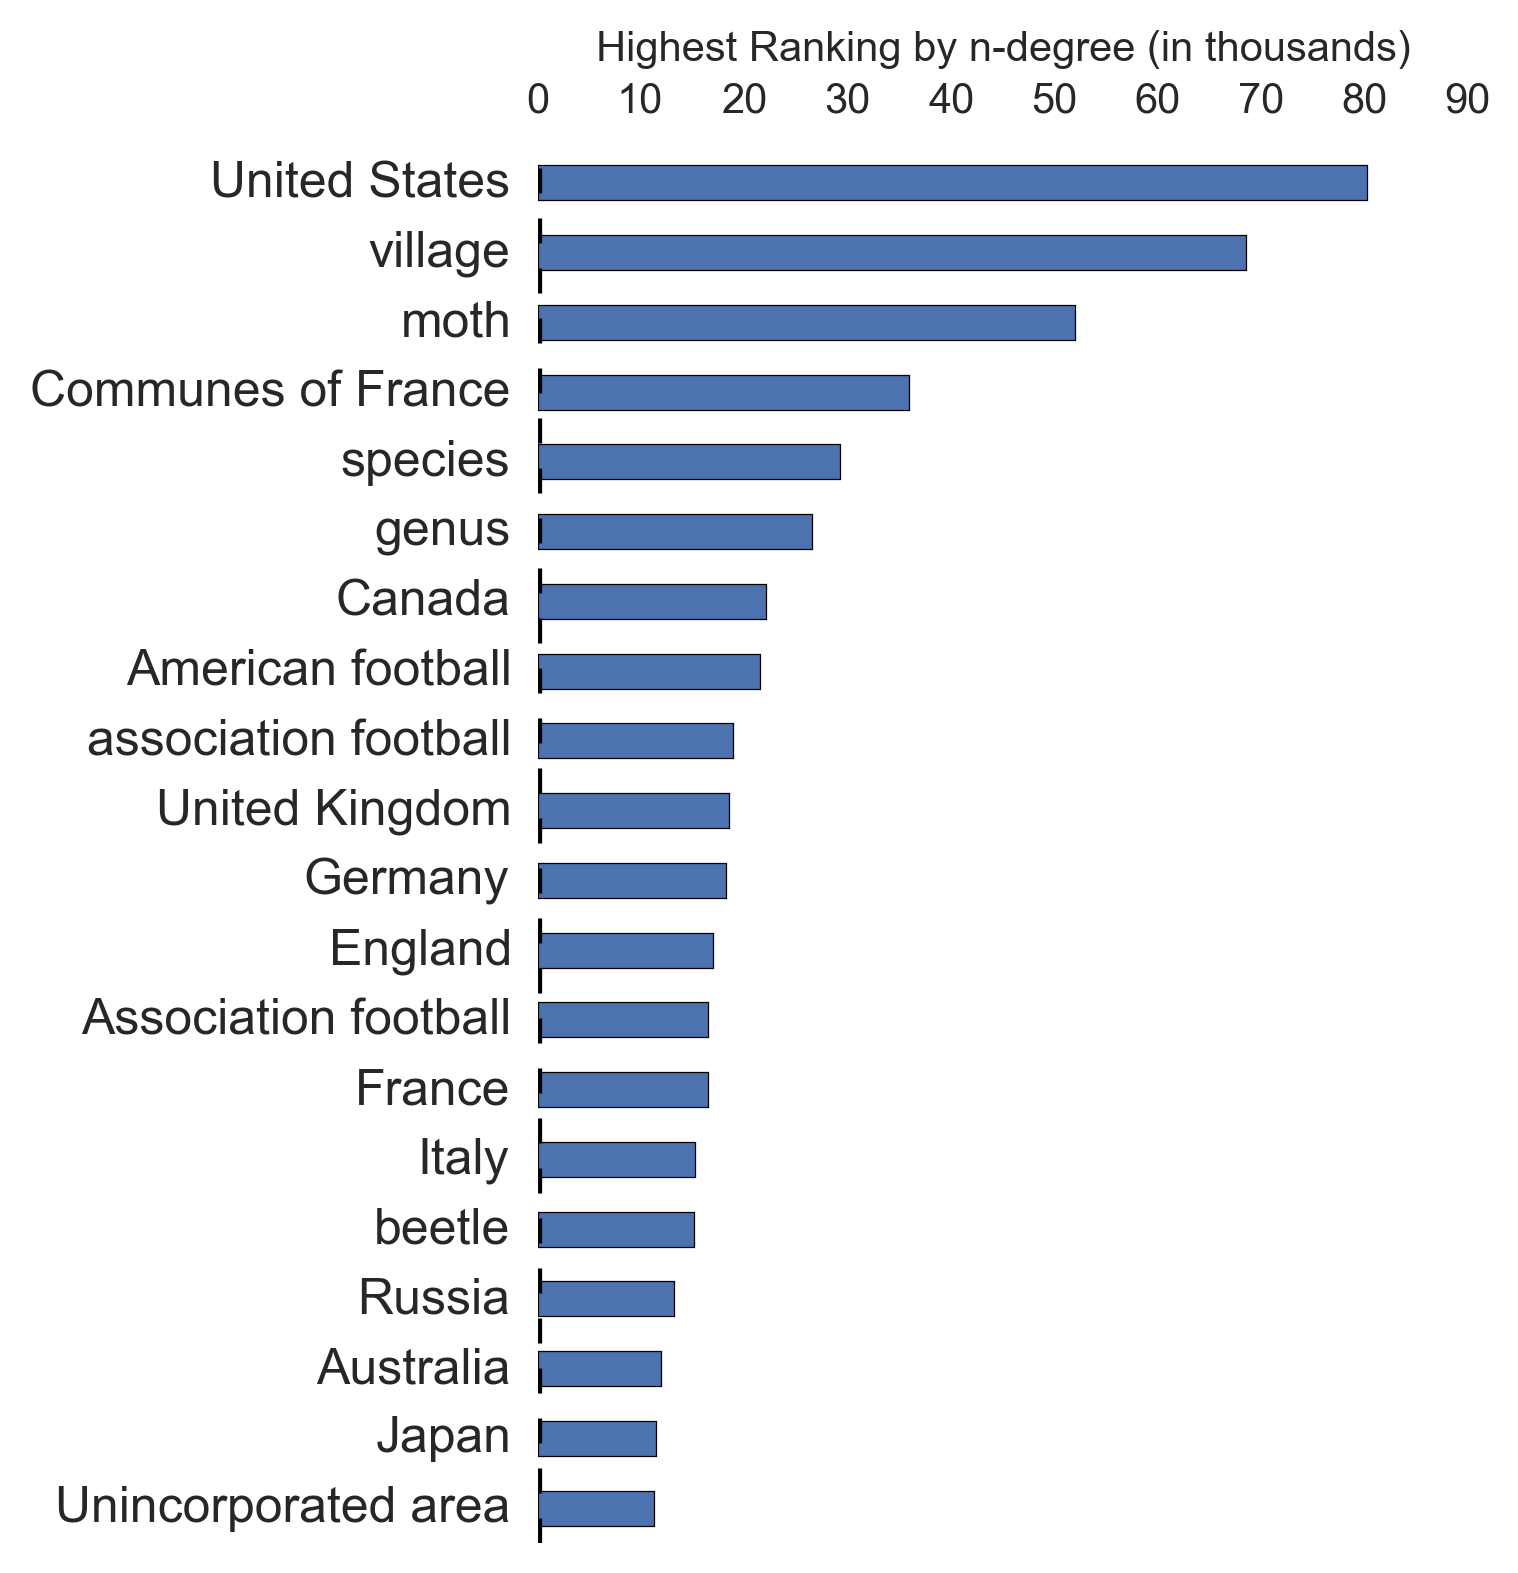
\includegraphics[width=\columnwidth]{graphics/articles_ndegree.png}
  \caption{
    \textbf{Highest Ranking Articles by indegree}
  }
  We rank each article by the number of direct first links to the article (indegree). The highest-ranking articles tend to represent abstraction for concepts
  comprised of various facets and parts.
  \label{fig:ndegree list}
\end{figure*}
We rank all 11 million articles by indegree to find 
the "United States" with 80,249 direct first links as the most referenced
Wikipedia article. 
Other high-ranking articles
include foundational abstract concepts such as "village," "species,"; 
sports associations such as "American Football," "Association Football"; 
and developed nations such as "France," "Japan," "Russia," "Australia," and 
the "Netherlands." These high ranking articles are useful abstractions: nations
describe a collection of individuals, a common culture, language, or 
geographical proximity; sports teams describe an ever changing collection of 
sports players often associated with a cultural identity and a geographical 
region. Since abstractions such as nations and teams are inherently comprised
of many parts, authors reference the larger abstraction when describing 
a part. For example, in describing the geographical region of north America, 
the United States, Canada, or Mexico are natural references anchoring the 
geographical location to a larger national identity. 

"Philosophy" and other philosophical concepts with many traversal visits
are not among the highest-ranking articles by indegree.
"Philosophy" has an indegree of 581, with direct first links from articles about Philosophers and areas of Philosophy: "Existentialism and Humanism," "Predeterminism," "Synoptic Philosophy,"Qualia," "Dorothy Emmet," and "Christopher W. Morris."
While many articles accumulate at "Philosophy" (see traversal visits discussion), 
the accumulation is not the 
result of many articles directly referencing "Philosophy." 
Instead, the accumulation of first links, as we argue in our 
discussion of traversal visits, flows towards Philosophy as the 
ultimate anchor when genralizing from specific articles towards broader notions.
\begin{figure*}[tp!]
  \centering	
  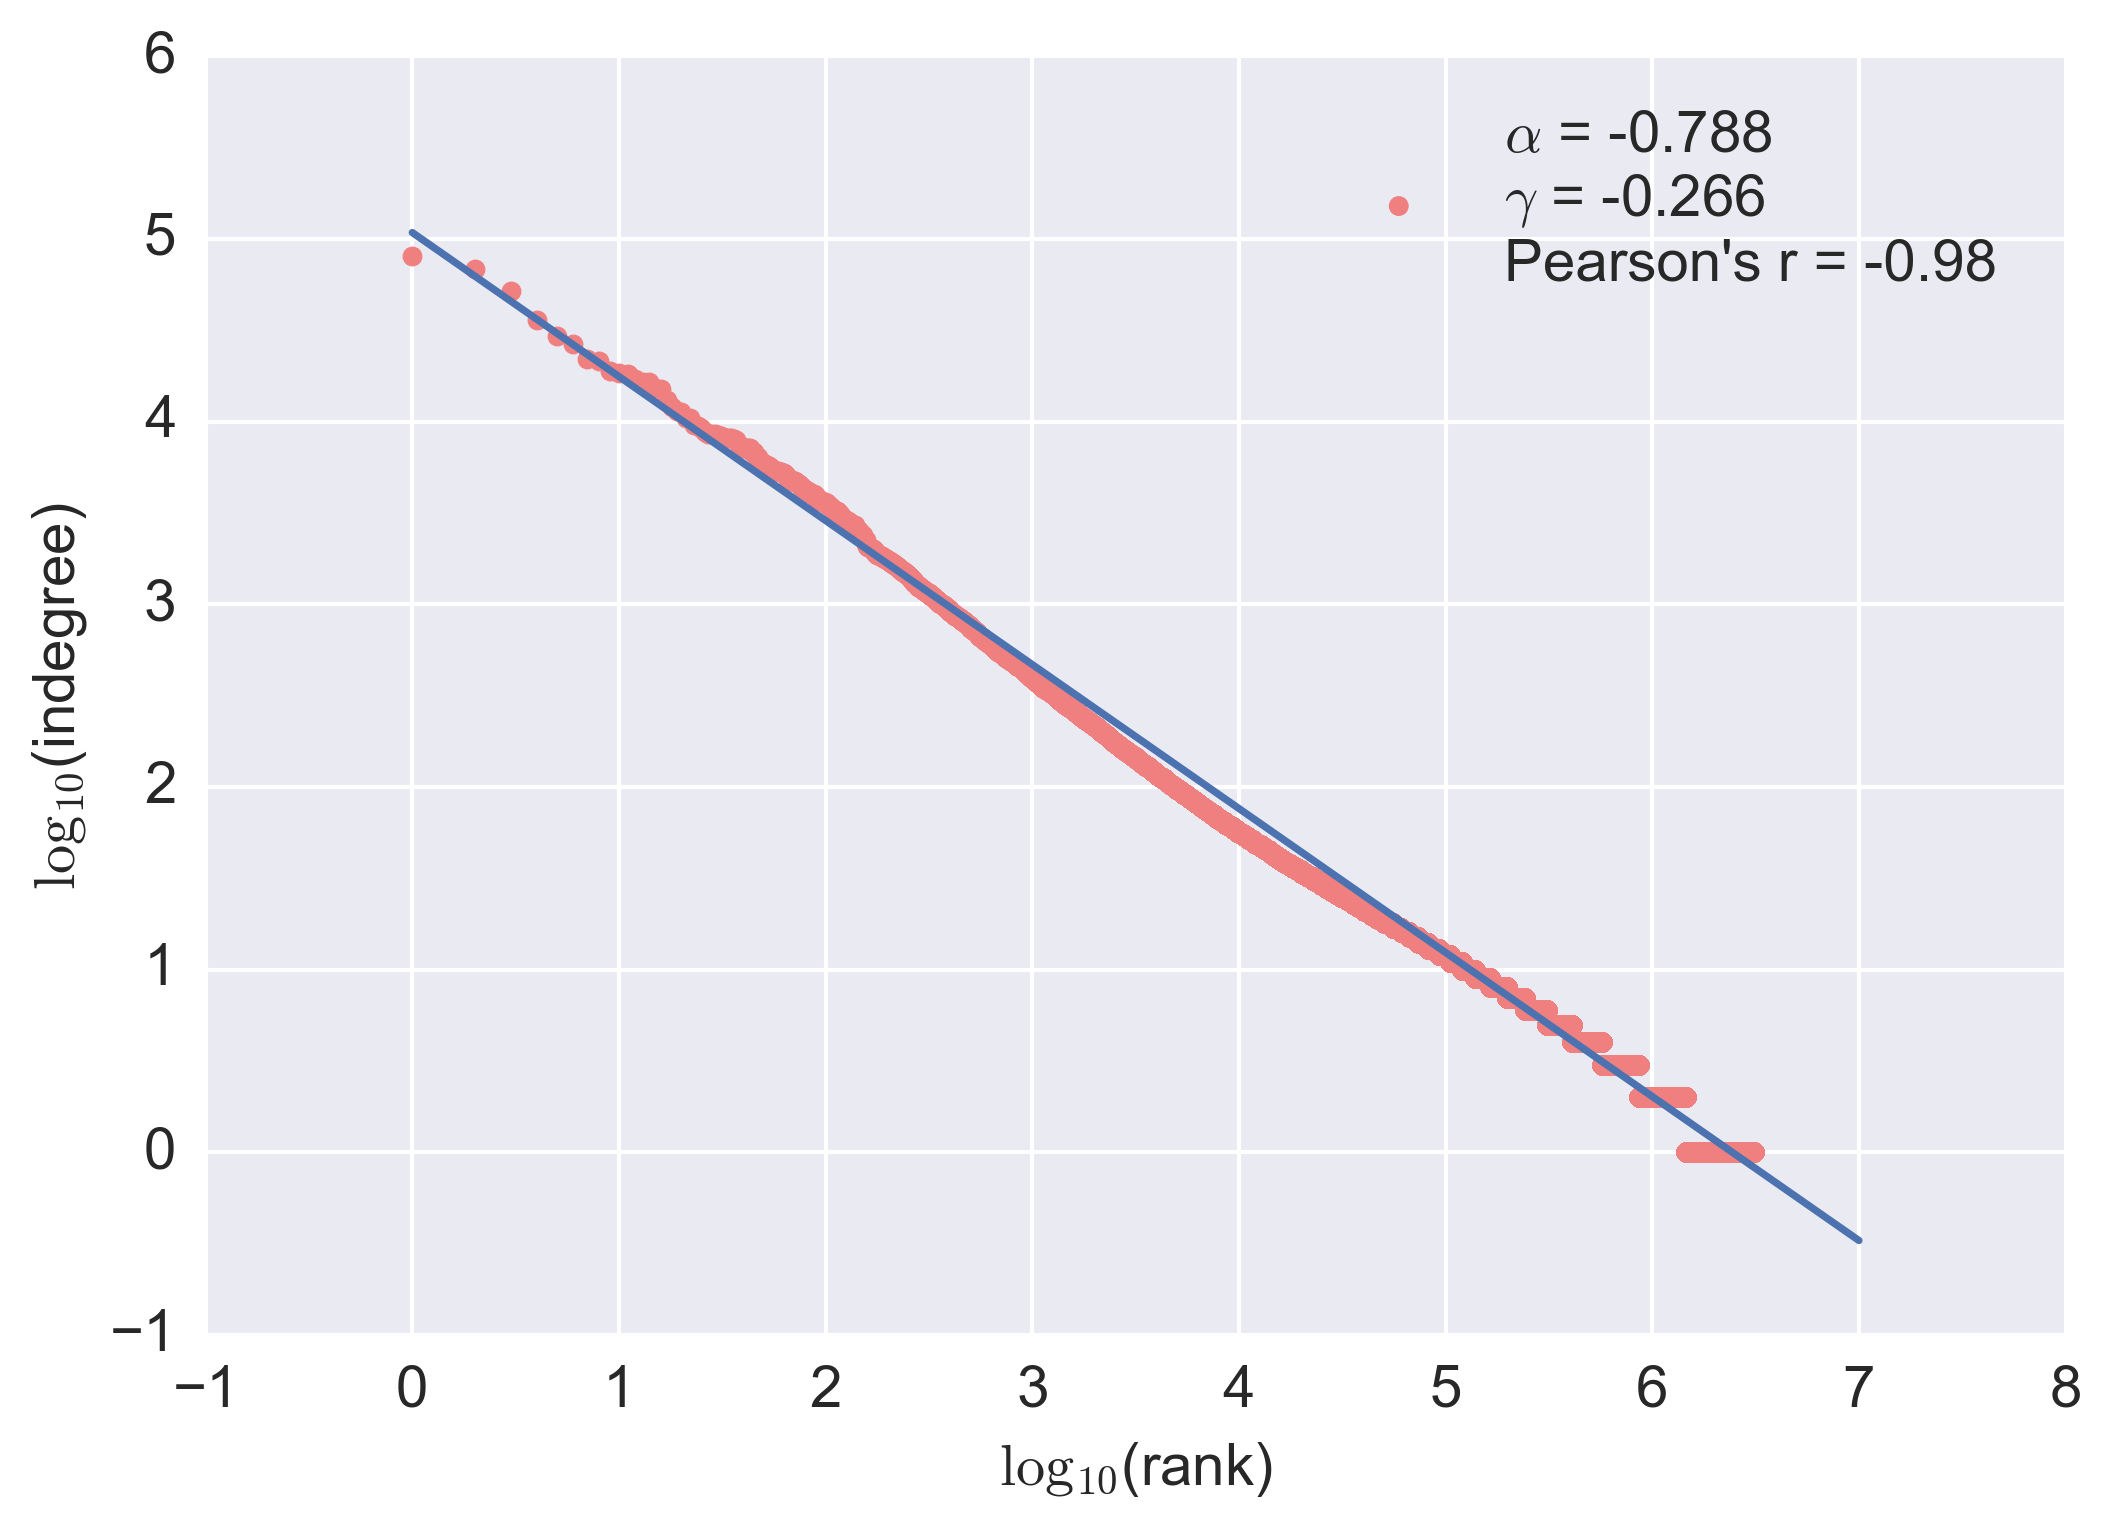
\includegraphics[width=\columnwidth]{graphics/ndegree_loglog.png}
  \caption{
    \textbf{FLN Degree Distribution}
  }
  We construct a log-log plot fit our results to a linear model. The result is a 
  an excellent fit with r = -0.98, yielding a power law exponent of -0.79. 
  The distribution appears scale free with most articles having fewer than 9 
  direct first links, while few hold most.
  \label{fig:degree distribution}
\end{figure*}
The FLN's indegree exihibits a scale-free distribution where a few articles 
receive a most direct first references, while most articles receive few or none.
The average indegree for all 11 million articles is 3.6 direct first links with a standard deviation of 89.5 links.
Only 4826 articles have more than 100 direct first links and $75\%$ of articles
have fewer than 9. 
When fit to a linear model on a log-log scale (log(rank) versus log(indegree)), 
the model's r value is $-0.98$ suggesting a strong log-log linear fit 
with a power law exponent of $-0.79$. 

\centerline{***}

Beyond indegree, our work expands the analysis of relations to understand 
how many more than two articles are organized and related. 
We develop the notion of a path to describe the structure of the FLN as a 
flow relating ideas. We traverse every possible path through the FLN, taking 
$232$ million steps along the way.


\subsection{Depth of the FLN}

We first seek to describe the depth of the FLN: how many links does a 
connection of ideas span? We gauge the FLN's depth via path length or the number of links traversed until a repeated or invalid link (one outside the FLN). 
We discover the longest path length is 365
corresponding to the yearly calendar of Orthodox Liturgics.
Each day's Liturgics link to the next day's. Curiously, on the last calendar day, the last article simply links back to January 1, forming a 365-cycle 
(see discussion of cycles).
We also found similarly lengthy paths following the evolution of a place or topic through time: 
"1953 in Scotland" or "1560s Architecture", with articles sequentially proceeding by year, decade or era.
The longest paths connecting ideas are organized temporally.

\begin{figure}[tp!]
  \centering	
  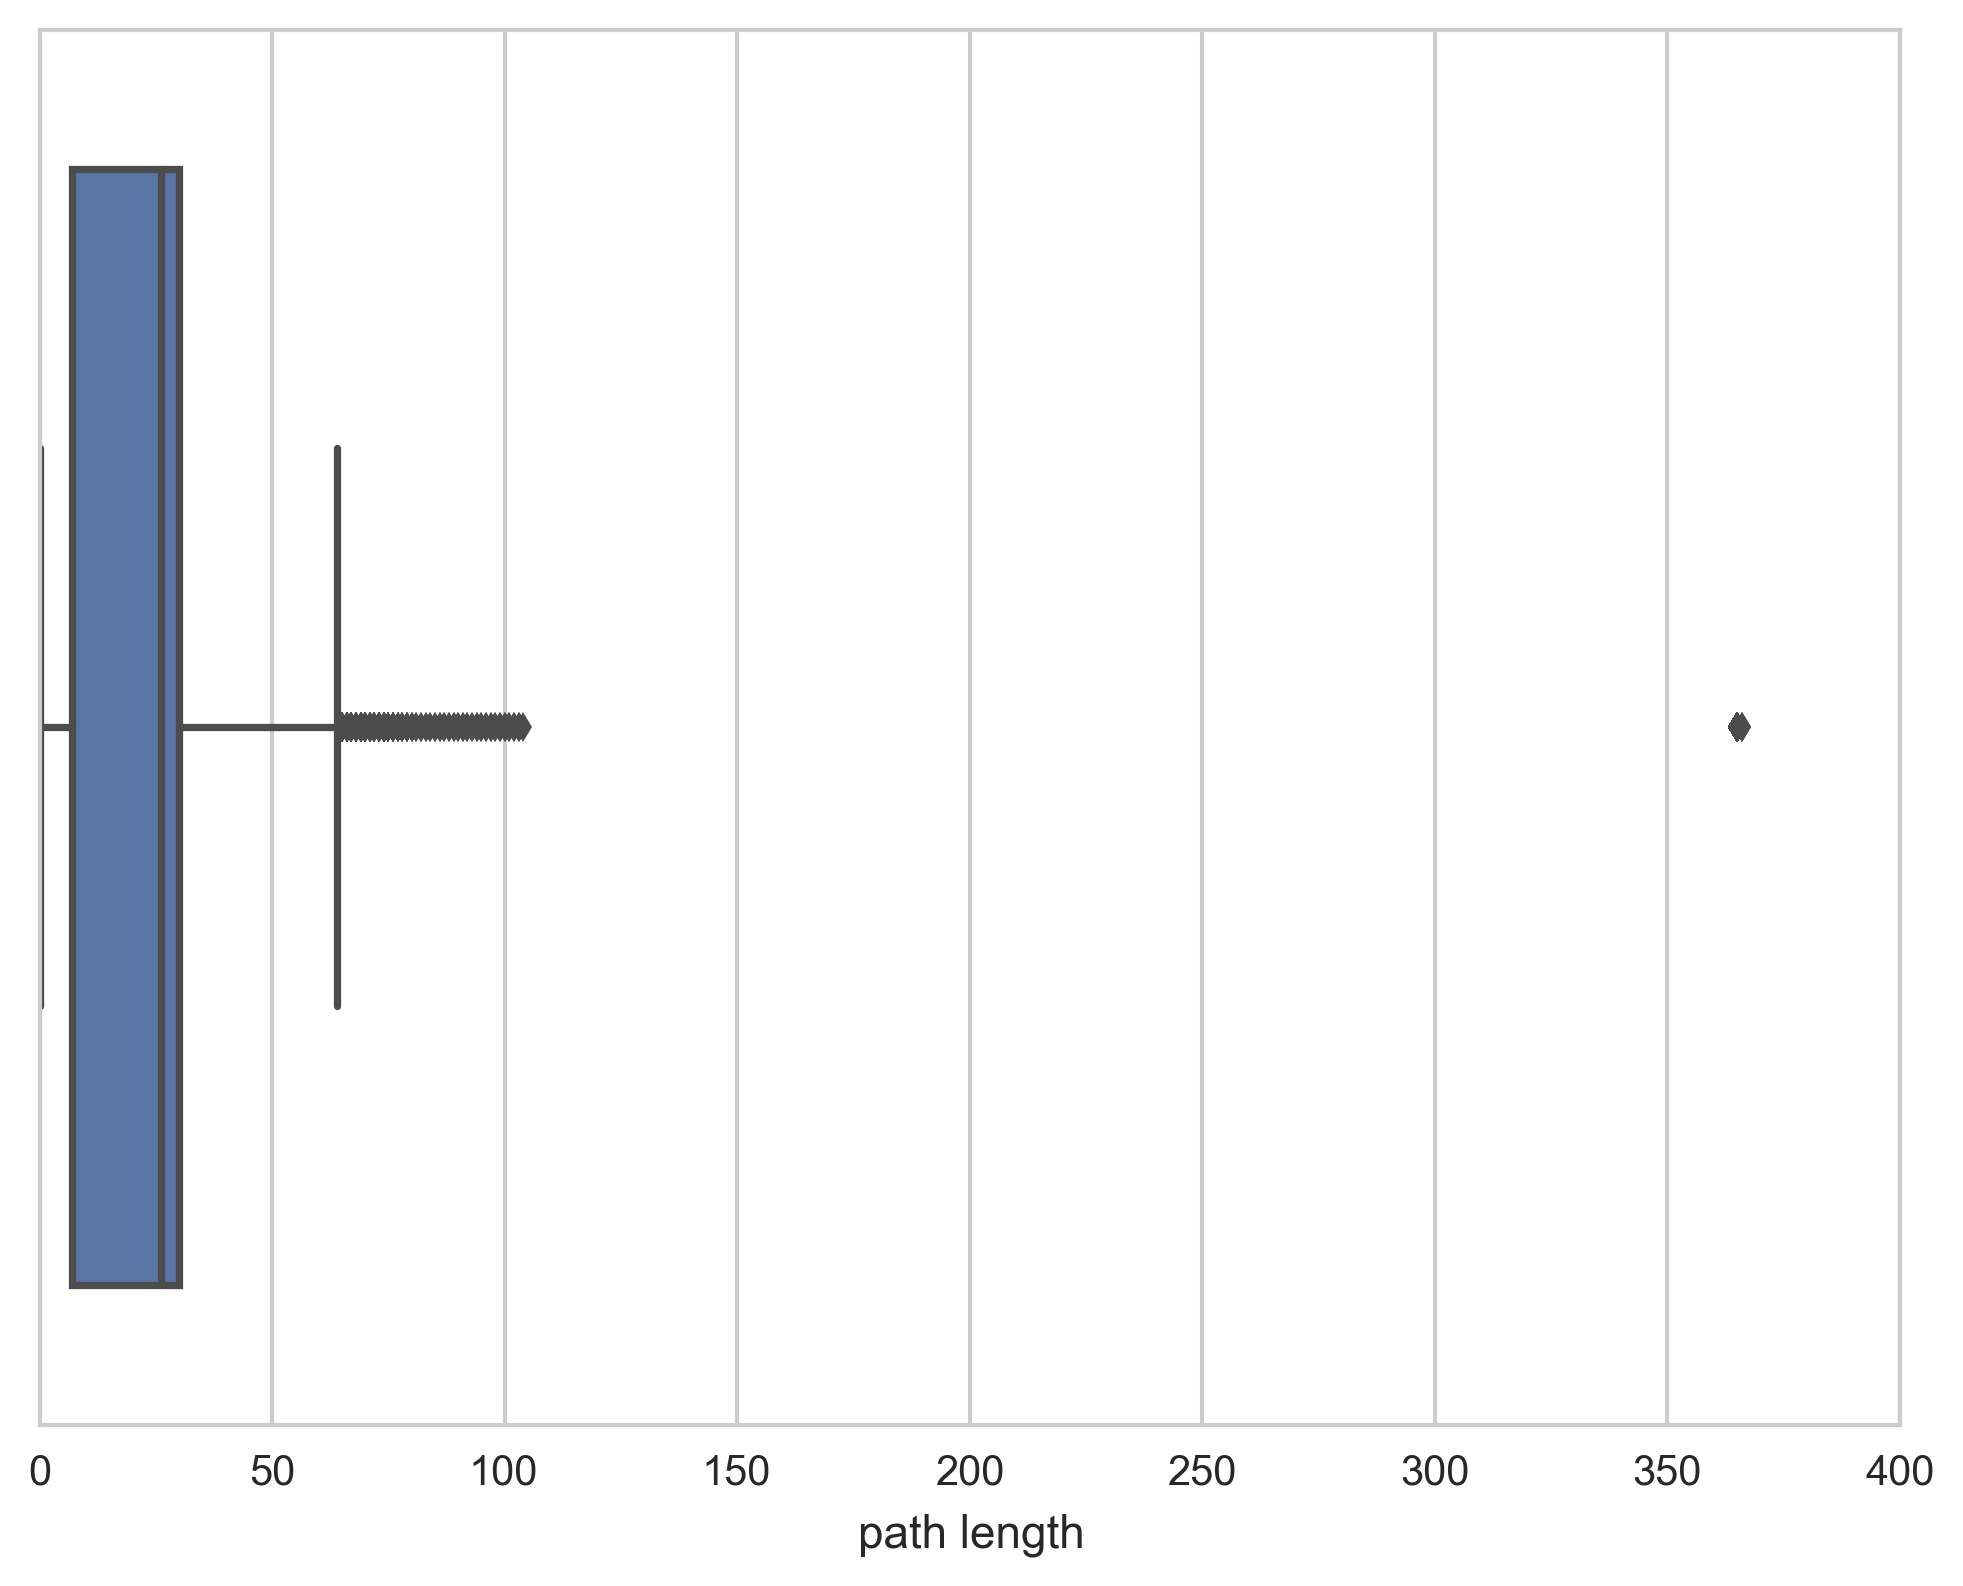
\includegraphics[width=\columnwidth]{graphics/path_lengths_boxplot.png}
  \caption{
    \textbf{Path Length Distribution}
  }
  The median network depth measured by the number of first links in a path
  is 29. The 365 cycle for "Orthodox" liturgics is the outlier to the right, while
  other historical articles about "Scotland," "UK" and so on are slightly outside
  the third quartile. More than $75\%$ of articles have path lengths between 
  $0$ and $50$ links.

  \label{fig:Path Length Distribution}
\end{figure}

Of the 11 million articles, 5.5 million had an invalid link or linked back to the same article, yielding a path length of zero. 
This roughly corresponds to the official number of articles on Wikipedia 
$~4.7$ million as of November 2014---approximately half of the 11 million 
articles in the XML dump are redirects or disambiguations, not full articles.
The most common path length is 29, with an interquartile range (26, 30).
The median path length far exceeds the popular 6-degrees of separation (see for 
example the average number of academic publications separating scholars 
\cite{six_degrees}), indicating a greater network depth. The network depth suggests a large network of spanning a variety of ideas.
As a distribution, more than $75\%$ of articles have a path length below 
$50$ first links 
while a few temporally organized paths exceed 50 links 
(see figure~\ref{fig:Path Length Distribution}). 
How can we characterize the flow of ideas along a path? Next, we develop 
a metric to gauge the accumulation first link references
and characterize a global organization 
of ideas among articles.




\subsection{Traversal Visits}

We followed every possible path through the network, incrementing
the number of traversal visits for every first link reference along a path 
to generate a total of 232 million traversal visits.

As a distribution, the number traversal visits per article appears scale-free. The majority of articles have fewer than 30 traversal visits, while few 
have 5 order of magnitude more traversal visits. 
Specifically, $99.76\%$ of articles have fewer than $100$ traversal visits; nearly $80\%$ have none. 
Meanwhile, the highest ranking 30 articles have an extremely disproportionate number of traversal visits.

\begin{figure*}[tp!]
  \centering	
  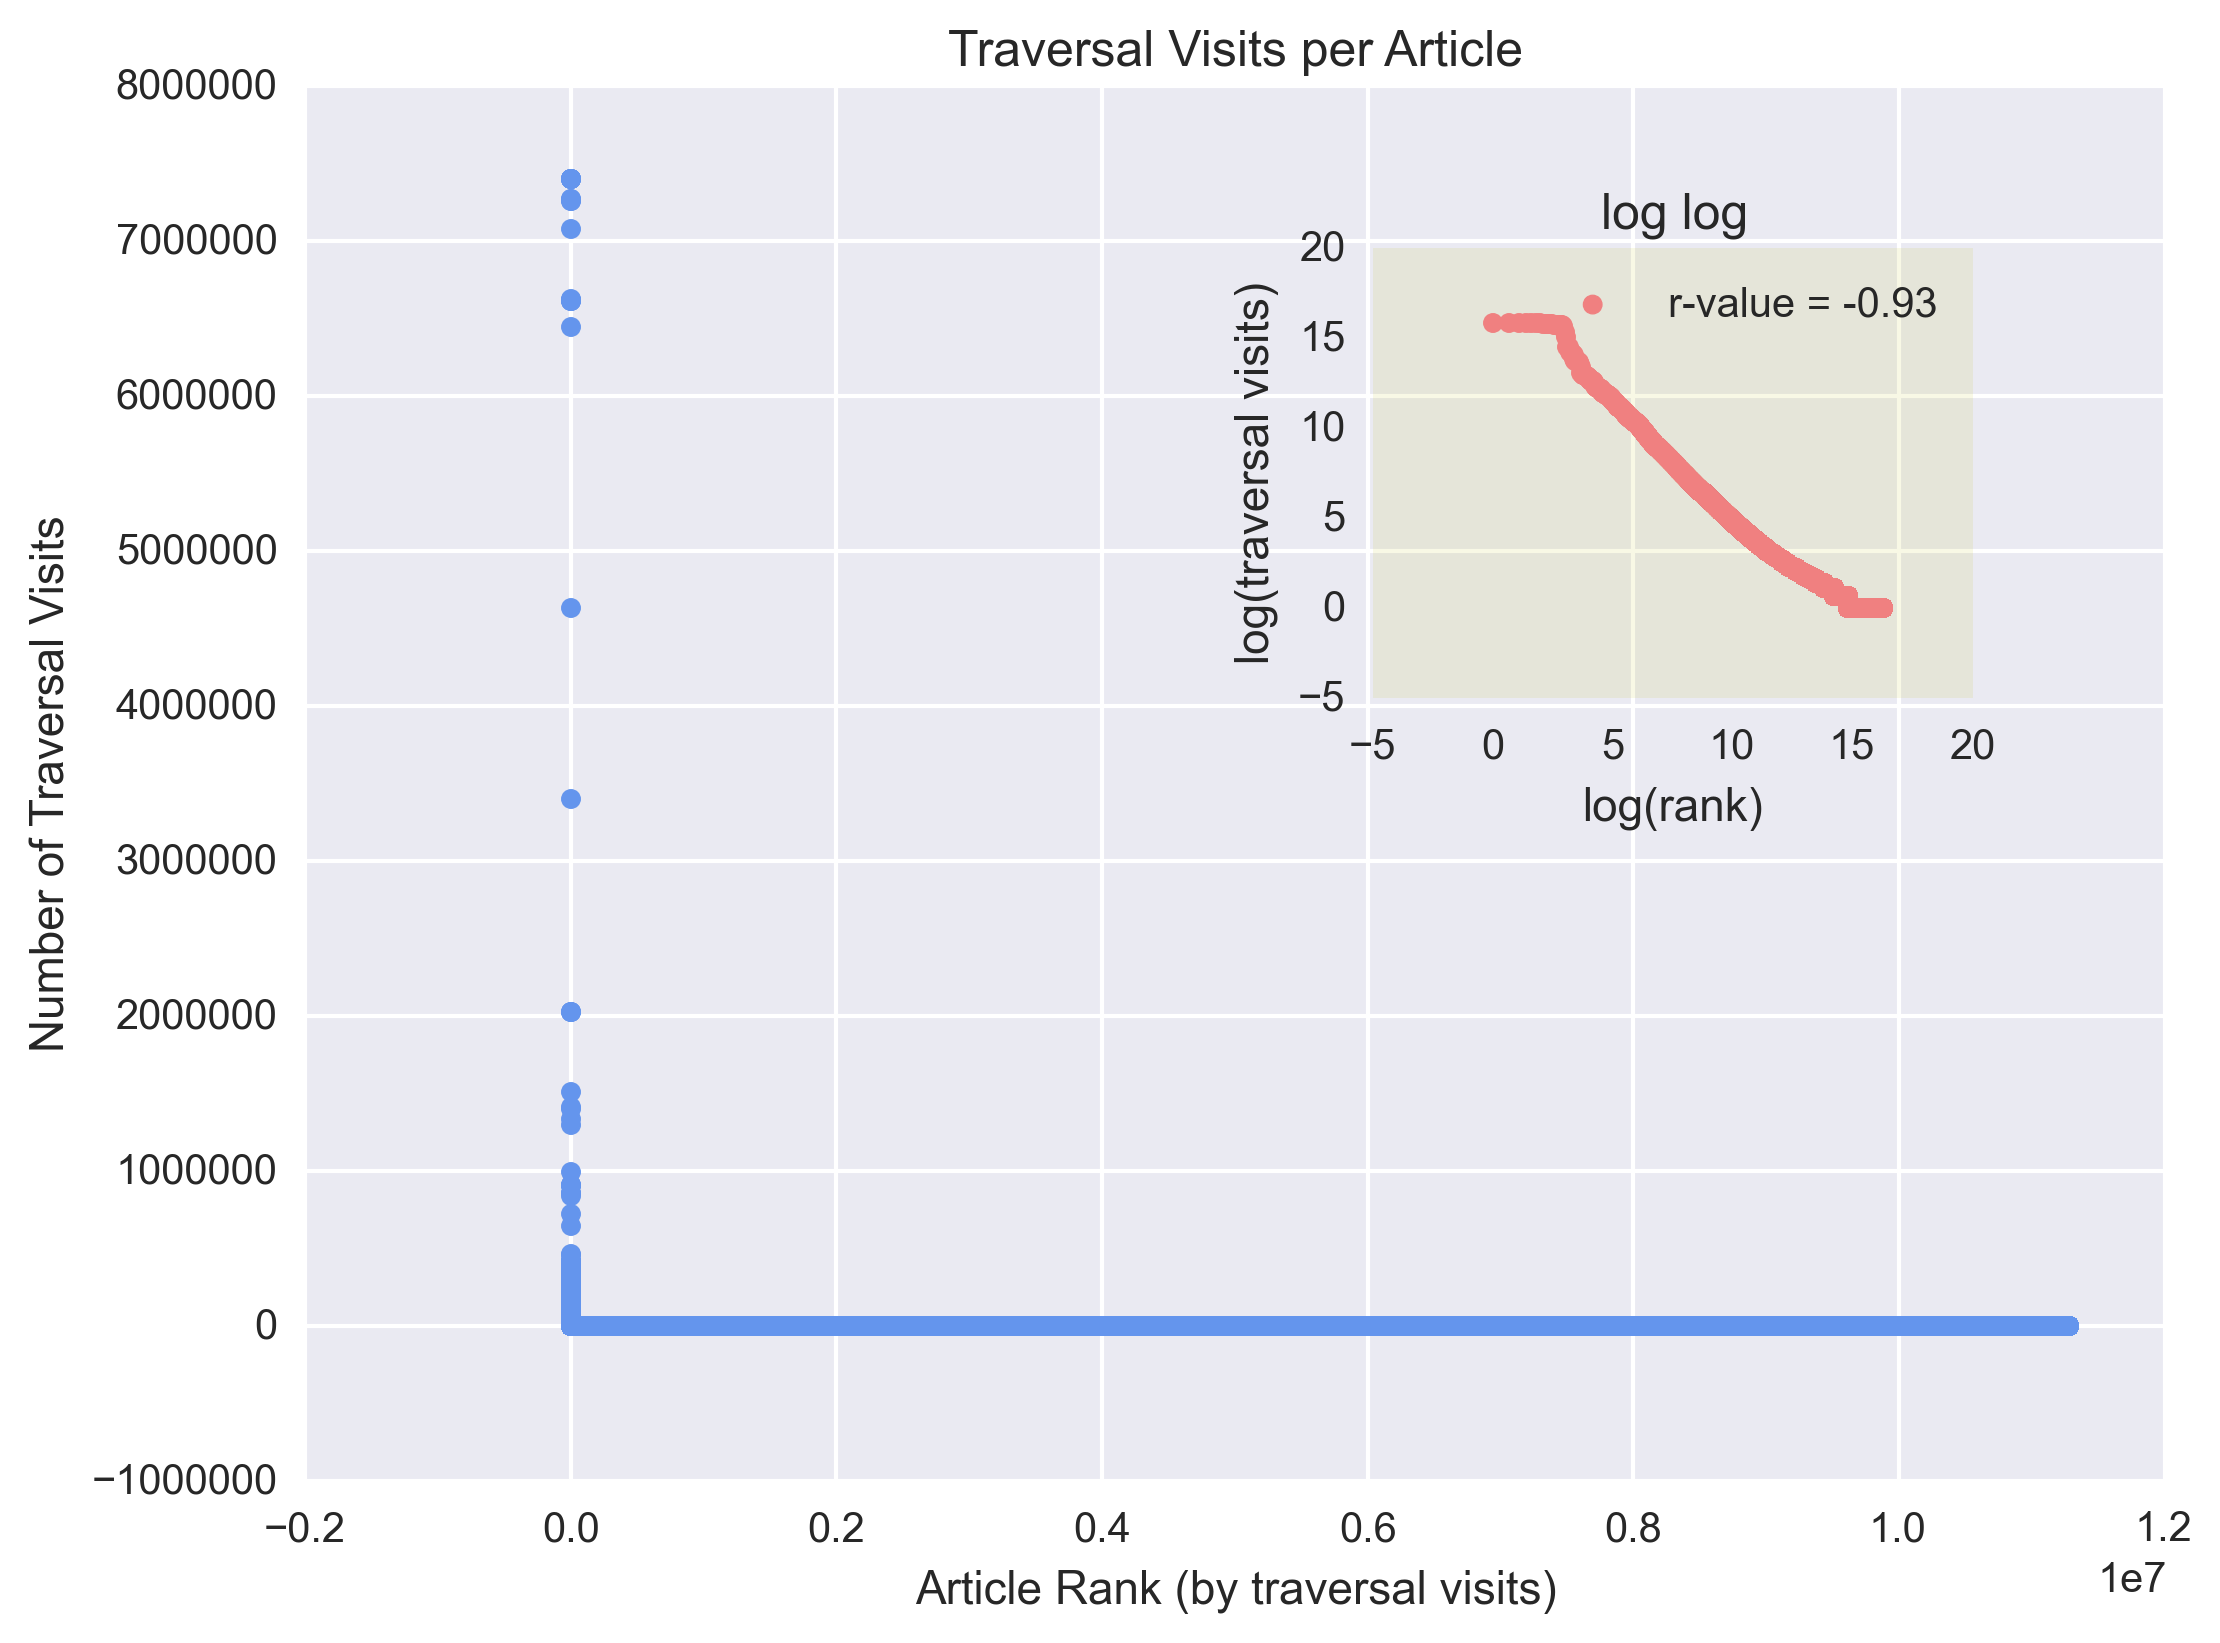
\includegraphics[width=\columnwidth]{graphics/traversals_per_article.png} 
  \caption{
    \textbf{Distribution of Traversal Visits}
  }
  We fit the distribution to a linear log-log model by considering the log (base 10) transformed rank of each article against log (base 10) transformed the number of traversal visits. 
  The model explains $86\%$ of the variation in the data, yielding an r-value of $-0.93$ 
  and a power law exponent of $-0.636$. The horizontal flattening around the highest
  ranking articles is a result of the cyclic structure (see discussion on cycles).
  \label{fig:Distribution of Visits}

\end{figure*}

To more accurately gauge the distribution, we construct a log-log plot of the entire dataset: log(traversal visits) against log(rank). We observe a fairly linear fit, as is characteristic of scale-free networks, with an r-value of -.93 and 
a power-law exponent of $-0.636$. A handful of the highest ranking articles contain a disproportionate number of traversal visits, while most have none. The skew in the distribution is not terribly surprising when considering the heuristic of how the links flow: from specific to general. 

The highest ranking articles include Philosophy alongside related articles such as "Existence", "Quality", and "Reality".

\begin{figure*}[tp!]
  \centering	
  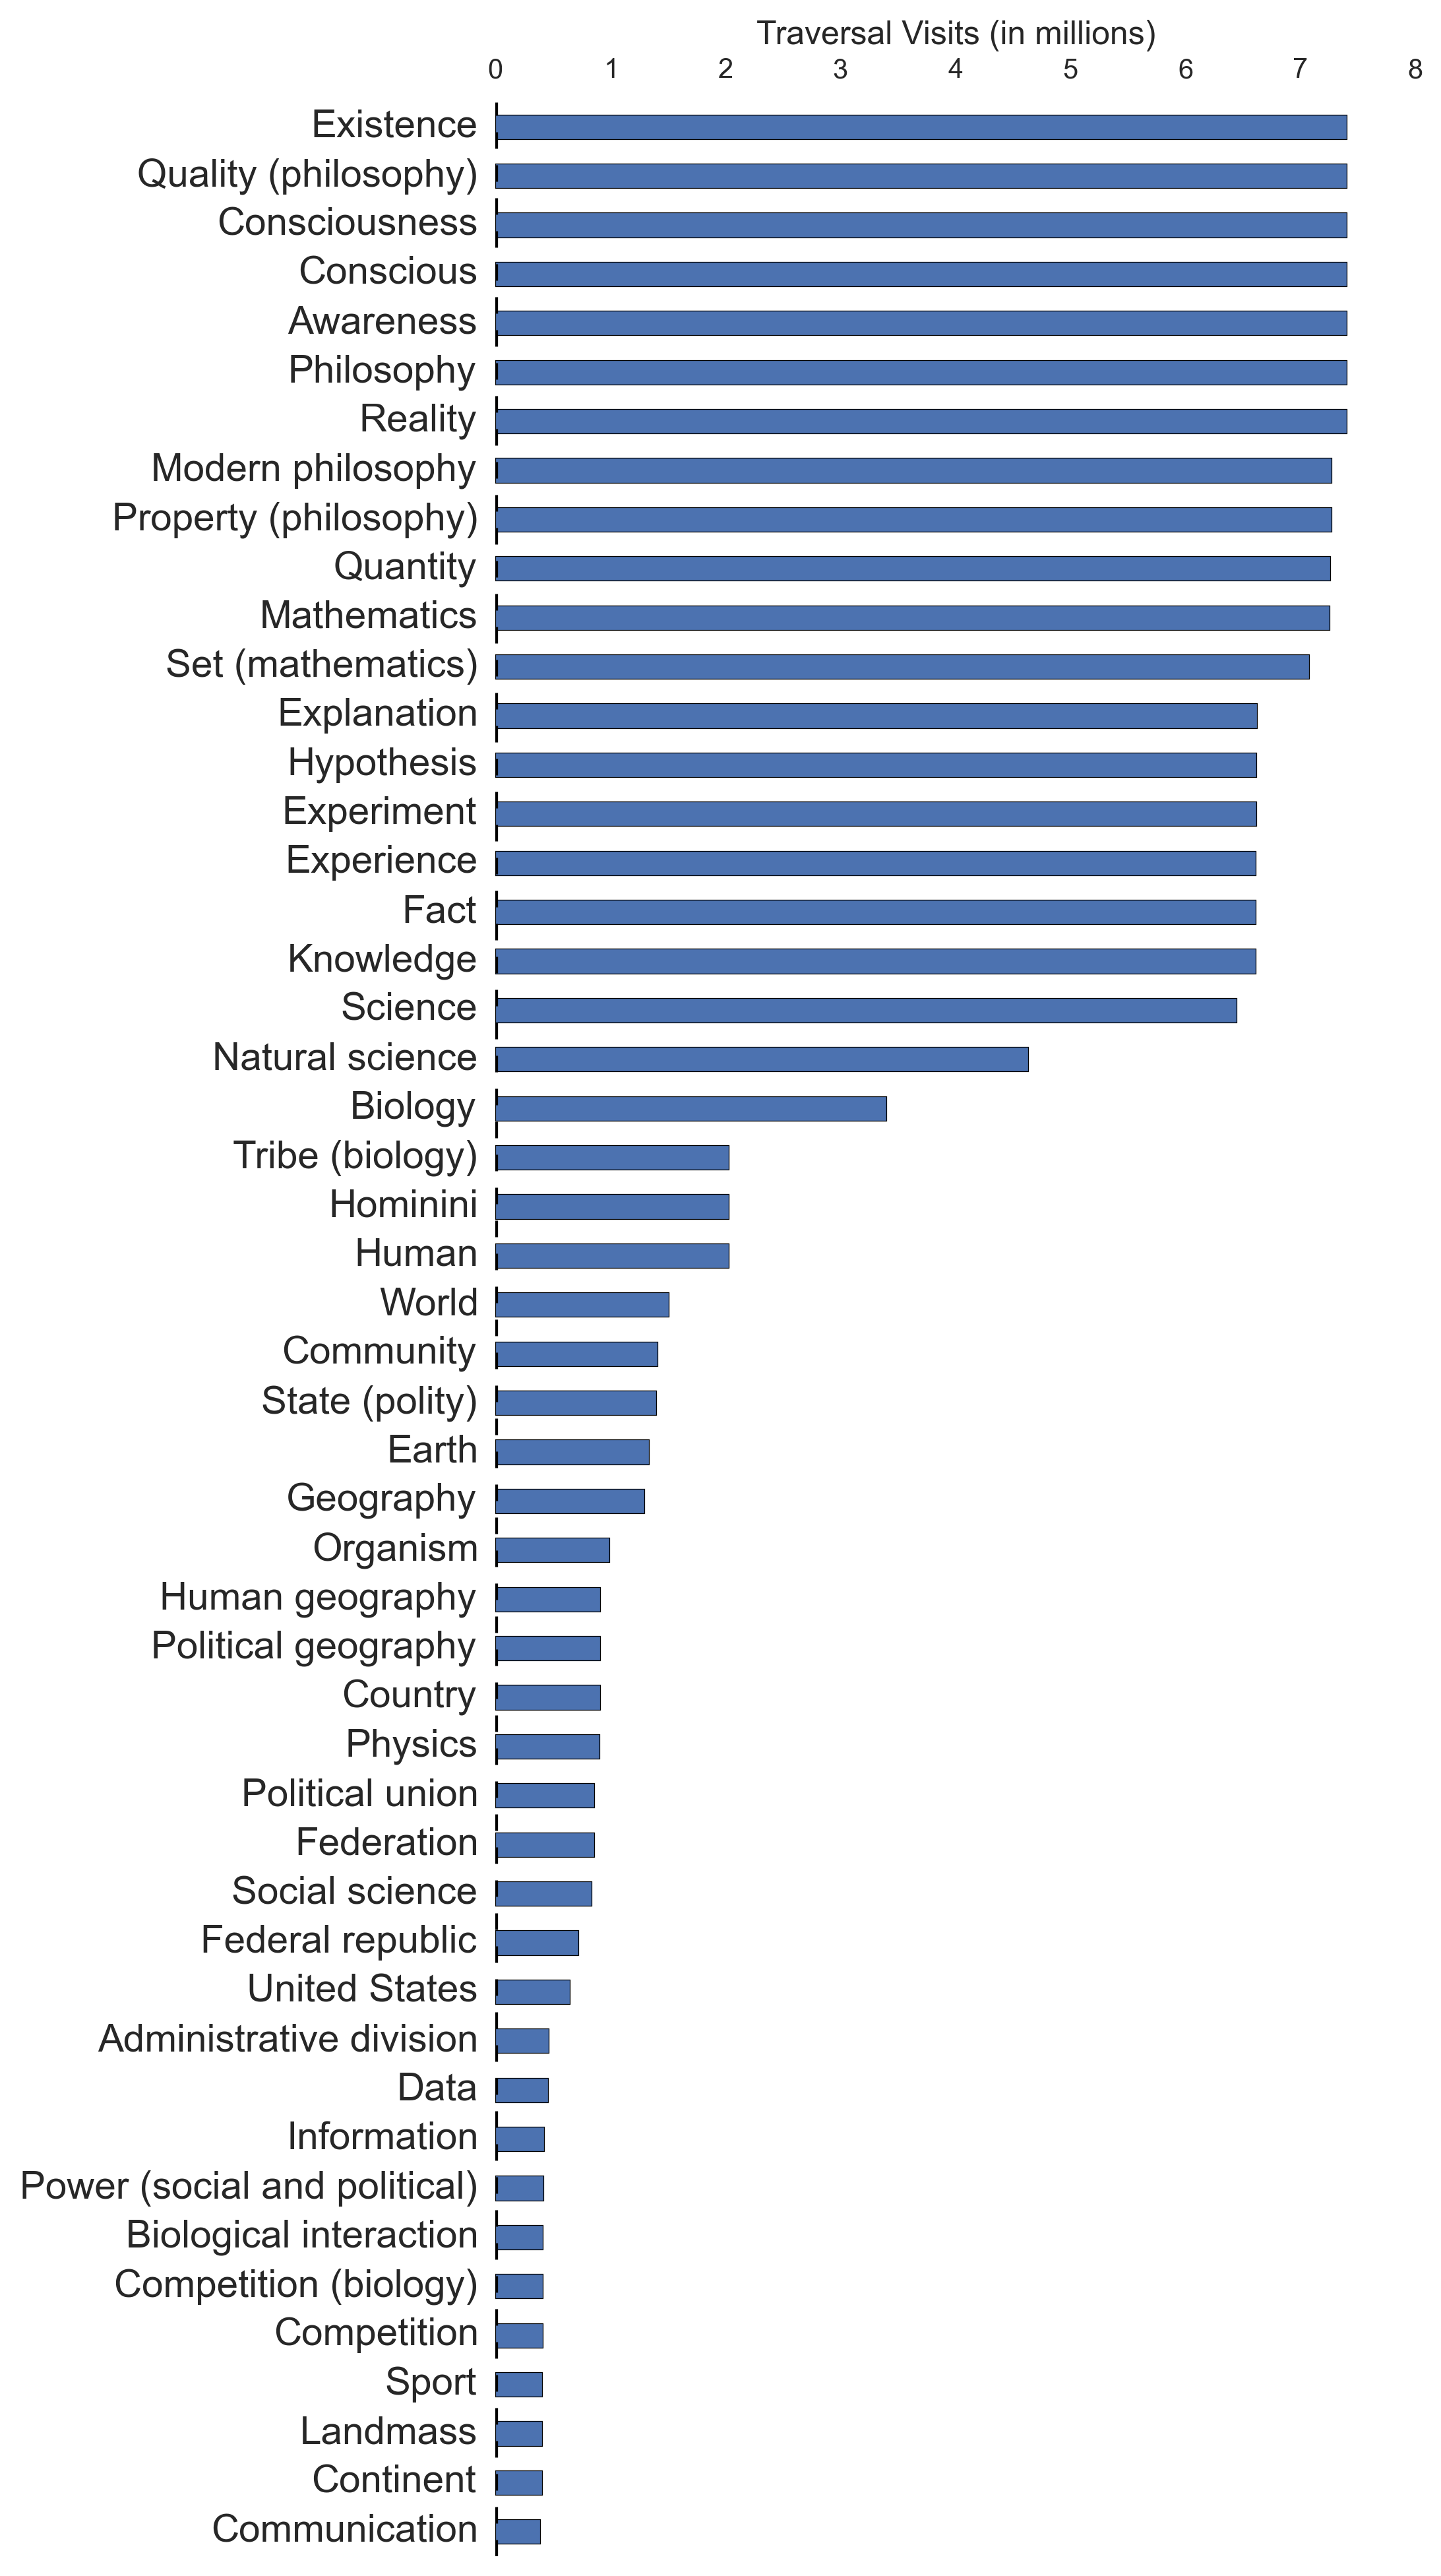
\includegraphics[width=\columnwidth]{graphics/articles_ranked.png}
  \caption{
    \textbf{highest ranking articles by number of traversal visits}
  }
  We compute the number of traversal visits for each article in the FLN (see 
  Traversal Algorithm section for details). In doing so, we can rank each article
  by the accumulation of first links. Articles with a greater number of traversal visits
  mark greater points of first link accumulation. The highest ranking articles by traversal visits reveals where the greatest accumulation occurs.
  \label{fig:highest visits}
\end{figure*}


\subsubsection{A flow from general to specific}

The highest ranking articles by traversal visits are 
broad, global topics: 
many are academic disciplines such as "Science," "Math," 
"Geography," "Biology," and "Physics"; others are abstract fundamental concepts such as 
"Community", "State", "Earth", "Information", "Communication", and "Power."
Since traversal visits measure the accumulation of First Link visits in Wikipedia, 
the highest ranking articles suggest a flow from specific to general. 
For example the flow of First Links for the "Banana" article begins at a very concrete
and specific topic then flows into progressively broader and broader disciplines, eventually 
culminating at "Philosophy: "Banana" links to the broader category of "Fruit," which then links to 
"Botany," eventually "Biology," then "Science" and ultimately "Philosophy." 

One means to measure the specificity of an article is to identify the number of synonyms available for a word or topic. The reasoning here is that a  broader topic likely has many more synonyms relative to a specific, concrete topic. Banana has fewer synonyms than botanical for example. To quantify the observed flow, we measured the number of synonyms the article title contained in WordNet---the largest lexical database of the English language 
\cite{wordnet}. 
We find the highest ranking 100 articles have on average 5 more synonyms than the typical article; a difference of 2.5 synonyms if we compare the median number of synonyms in each group. 
As suggested by the median, many articles have no synonyms as we might expect, because titles with more than one word are not likely to appear in a thesaurus. 
Since many articles have no synonyms, we also compared the number of synonyms in the highest-ranking versus typical article, this time excluding all articles without at least 1 synonym. 
We still find the highest ranking 100 articles with an average of 9.0 (median of 7.0) synonyms whereas the remaining articles on average 5.8 synonyms (median of 7.0), even with the exclusion of all articles without any synonyms.
The quantifiable difference in synonyms corroborates the flow of links from concrete, specific articles to broader disciplines or fundamental notions.




\subsection{Network Cycles}

The recurrence of an exact number of traversal visits suggests some articles are part of a cycle. 
The "Philosophy" article for example sits in what seems like a cycle of seven other articles; "Hypothesis" appears to sit in a 
cycle of 6 other articles including "Experiment", "Fact", and "Knowledge".
To confirm the suggested cyclic structure, we record the history of articles traversed along a path. For example starting on "Train" we construct an path of articles: 
"Rain Transport,"
"Conveyance of Passengers and Goods," 
"Goods," 
"Economics,"
"Social Science,"
"Academic Disciplines,"
"Knowledge,"
"Awareness,"
"Consciousness,"
"Quality,"
"Philosophy."

We first identified 2-cycles, meaning a pair of articles with First Link pointing to one another.
Of the 11 million articles, 84,000 are 2-cycles. 
The highest ranking 2-cycles by traversal visits tend to be synonyms (or nearly so) rather than different, yet connected ideas:
"Health Care" and "Medical Case Management", "Broadcasting House" and "BBC", "Secondary Education" and "Secondary School".

\begin{figure*}[tp!]
  \centering	
  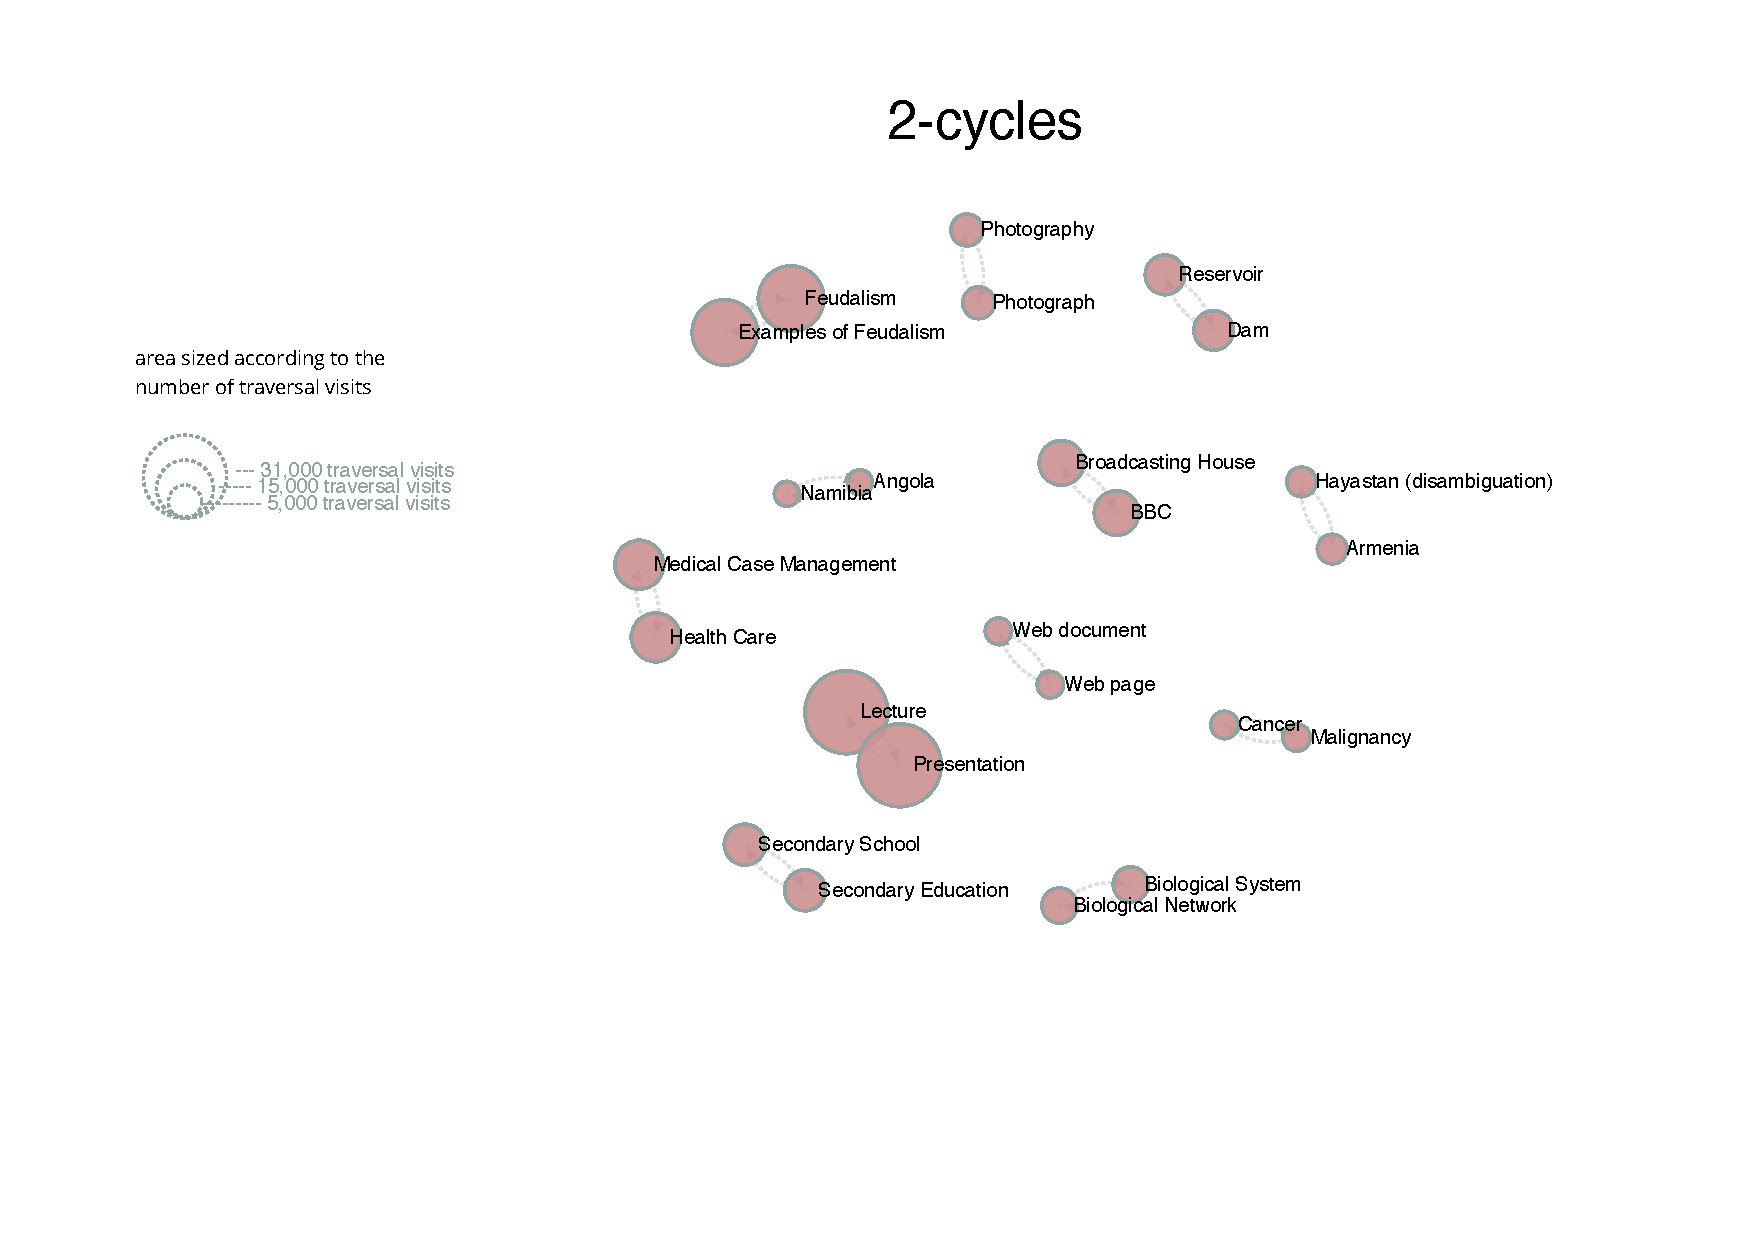
\includegraphics[width=\textwidth]{graphics/2_cycles.pdf}
  \caption{
    \textbf{highest ranking 2-cycles}
  }
  \label{fig:2-cycles}

\end{figure*}

Outside of the highest ranking 2-cycles, the typical 2-cycle signals a connection between different, yet very closely related ideas. 
Link patterns such as inventor to product ("Voere" to "VEC-91"), event to organizer ("Poetry Bus Tour" to "Weave Books"), and book to author ("Anatomy of Britain" to "Anthony Sampson").

Similarly, 3-cycles captured a synonymous or close relation among 3 articles: "Tree of life (Biology)", "Tree of life (disambiguation)", 
and "Tree of life"; "Cinema of India", "Indian Cinema", and "Telugu Cinema". Once we extend our cycle size beyond a length of 6 however, 
"Philosophy" along with the remaining list of high ranking articles by traversal visits dominate.

\begin{figure*}[tp!]
  \centering	
  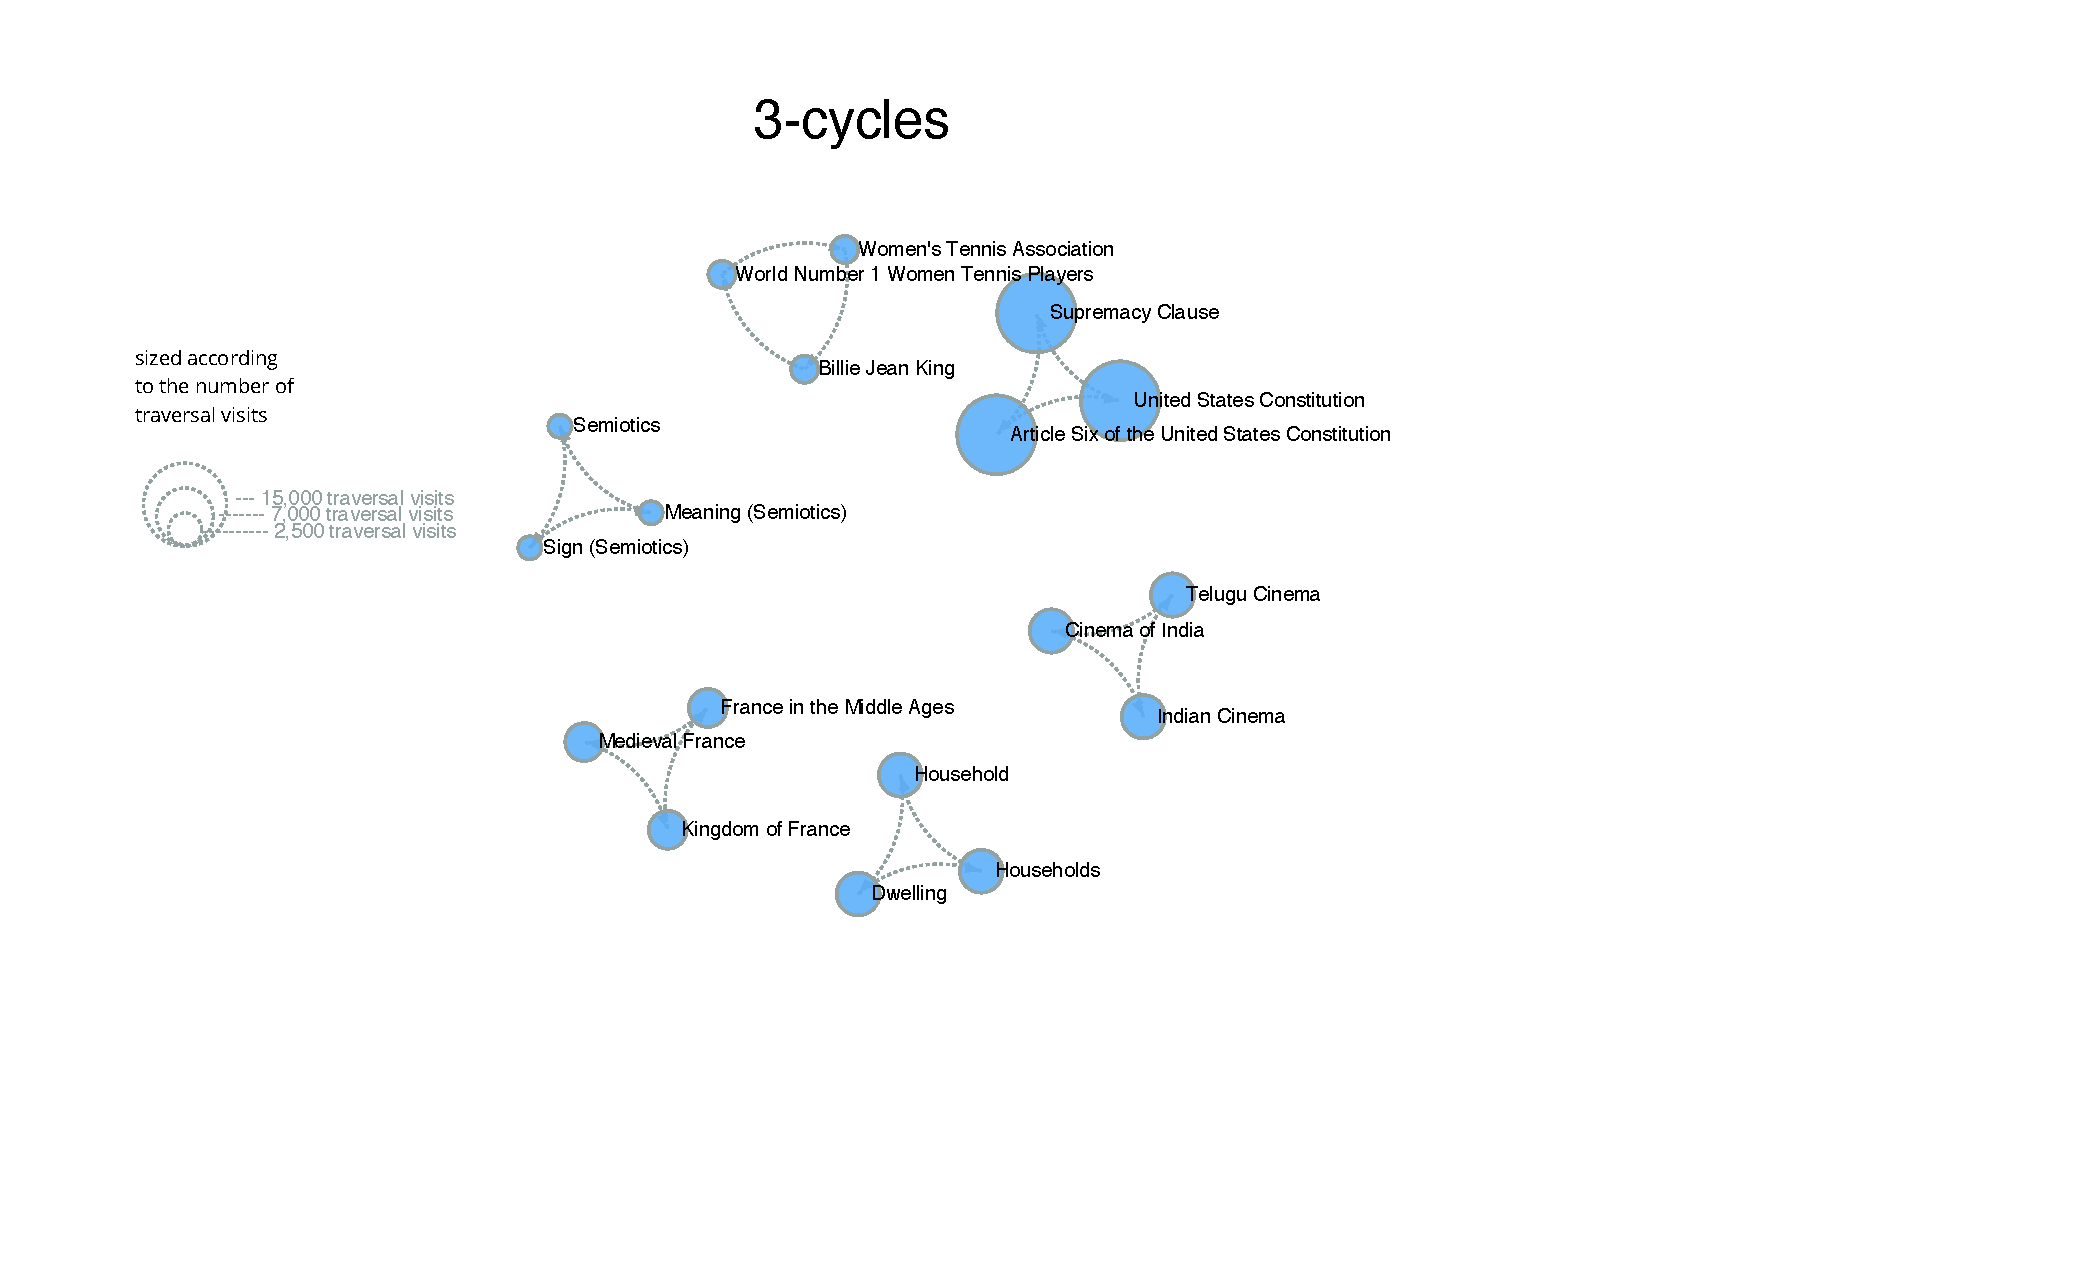
\includegraphics[width=\textwidth]{graphics/3_cycles.pdf}
  \caption{
    \textbf{highest ranking 3-cycles}
  }
  \label{fig:3-cycles}
\end{figure*}

The longest cycle in the network spans 365 articles of Eastern Orthodox Liturgics for each calendar day. 
Curiously, on the last calendar day, the last article simply links back to January 1, forming a 365-cycle.
Other lengthy cycles span 60-75 articles including collections of articles on national histories such as "Japanese Eras" 
or judicial bodies such as the "Legislative Assembly of Ontario".





\subsection{Basins}

We can group articles lying on the same path to identify {\it basins}: 
a group of path-connected articles.
Since cycles identify only groups of articles with a closed set of links, 
we additionally measure and rank basins to capture groups of closely related
articles branching outside of a cycle into the rest of the FLN.
We rank basins by the total number of traversal visits in each of the articles
along the path forming the path.
Akin to river networks, these basins are areas of accumulation with a path 
flowing outwards to the rest of the FLN.

The highest ranking basins by the number of traversal visits are groups of articles
around "Philosophy." 
Since the accumulation of first links to "Philosophy" is so high, 
the paths leading to "Philosophy" carry many references.
The highest ranking paths include branches of philosophy flowing through 
"Awareness,"Existence," and "Consciousness" to "Philosophy." Other paths
include concepts around "Mathematics," scientific "Experiments," 
"Biology," and "Fact."
These paths link many specific articles to "Philosophy," each funneled through a particular domain.

Excluding basins around "Philosophy" we find other basins around 
foundational ideas such as "Community," "Landmass," "Federal Government," 
"Presentation," and "Belief System." 
The basins around each of these foundational notions are 
various paths containing related articles. For example around 
"Community" we find basins
flowing from "United States" to "Federal Republic" to "Political Union" to "State" culminating at "Community"; we also find basins flowing from 
"Public Policy" to "Executive (government)" to "Government" to State" and then 
to "Community"; we also find paths flowing through a similar chain beginning
with "Democracy," another beginning with "Constitution," another at 
"Dictatorship," and so on. The ideas build from specific means of organizing
a community (or society) then build up to "Community." 
Other basins around landmass for example begin at specific geographical regions
such as "Eastern Europe" building up to "Continent" and finally "Landmass."
Each basin accumulates first link references through various 
natural paths linking general themes to the foundational concept.

Which specific articles direct the path towards a particular concepts? 
Next we study the FLN using traversal funnels to understand the influence
a particular article exerts in directing the flow of first link references.


\subsection{Traversal Funnels}


To analyze the influence of an article exerts in shaping the 
struture of the FLN, we measure the number of traversal 
funnels, or paths the article directs towards a cycle (or invalid links).
Articles directing more paths exert a greater influence over the structure
of the FLN by increasing the accumulation of first links in a particular
basin. To distinguish between an article 
that simply happened to fall within a cycle from an article funneling 
many first links, we 

To measure traversal funnels, we traverse the FLN in the same manner as we 
did for traversal visits, but end a path once we enter a cycle.
We are then able to distinguish between an article related to many other ideas
only by virtue of its place in a cycle from an article exerting influence over where the first links flow. 
An article with a large number of traversal funnels directs many references
towards a particular path. In our sample network 
(see figure~\ref{fig:Traversal Funnels}) article C 
directs the flow of links towards the 3-cycle, while articles A and B are 
receipients of the flow---without exerting any influence themselves. 
While articles A, B, and C all have the same number of traversal visits, 
article C has 4 traversal funnels (A and B have none). By incrementing the count of 
first link references on paths only up to a cycle, we can identifying which articles
exert the greatest influence over the network's structure.

By studying the FLN not only as collection of directly linked pairs of articles, but
as a flow of paths, 
we build a powerful arsenal of information with which to study the FLN. 
From accumulated references, cycles, basins to influence, we can measure how the many articles in Wikipedia are organized and related.





